\documentclass[12pt,a4paper]{article}

%--- font và tiếng Việt ---
\usepackage[utf8]{inputenc}
\usepackage[T5]{fontenc}
\usepackage[vietnamese]{babel}

\addto\captionsvietnamese{%
  \renewcommand{\figurename}{Hình}%
  \renewcommand{\tablename}{Bảng}%   
}

\usepackage[T1]{fontenc}      % better font encoding
\usepackage{textgreek}        % allows \textmu etc.
\DeclareUnicodeCharacter{03BC}{\ensuremath{\mu}}     % maps U+03BC → \mu
\DeclareUnicodeCharacter{0307}{\d{}}                  % maps dot‑below accent
\DeclareUnicodeCharacter{0304}{\=}
\DeclareUnicodeCharacter{0303}{\~}

%--- công thức toán học ---
\usepackage{amsmath}
\usepackage{amssymb}

\usepackage{enumitem} % Gói này giúp tùy chỉnh danh sách

\usepackage[most]{tcolorbox}
\tcbuselibrary{skins,breakable}

% Hộp chung cho code hoặc hình, tự co giãn
\newtcolorbox{flexbox}{
  enhanced,
  language=R,
  breakable,                % cho phép xuống trang mới nếu nội dung dài
  colback=blue!10!white,    % nền nhạt
  colframe=blue!60!black,   % viền đậm
  arc=4pt,                  % bo góc
  boxrule=0.8pt,            % độ dày viền
  left=4mm, right=1mm, top=1mm, bottom=1mm,  % padding
  title=\texttt{Result},   % tiêu đề (tuỳ chỉnh)
  fonttitle=\sffamily\bfseries,
  coltitle=white,
  colbacktitle=blue!60!black
}

%--- căn lề ---
\usepackage[left=2cm,right=2cm,top=2cm,bottom=2cm]{geometry}

%--- chèn hình ảnh ---
\usepackage{graphicx}
\usepackage{float}

\usepackage{geometry}
\usepackage{tikz} % Để vẽ khung bìa
\usetikzlibrary{calc}

\usepackage{longtable}
\usepackage{array}

% Cấu hình lề trang để bảng hiển thị rộng rãi hơn
\geometry{
 a4paper,
 total={170mm,257mm},
 left=20mm,
 top=20mm,
}


% Cấu hình lề trang
\geometry{top=2cm, bottom=2cm, left=2cm, right=2cm}

% 1) Cần trong preamble:
\usepackage{xcolor}
\usepackage{listings}
\usepackage[most]{tcolorbox}
\tcbuselibrary{listings,skins}

% 2) Định nghĩa môi trường codebox
\newtcblisting{codebox}{
  listing only,
  listing options={
    language=R,
    literate=
    % cho phép hiển thị dấu hash trong code
    {á}{{\'a}}1
    {à}{{\`a}}1
    {ả}{{\v a}}1
    {ạ}{{\d a}}1
    {ấ}{{\'{\^a}}}1
    {ẩ}{{\v{\^a}}}1 
    {ẫ}{{\~{\^a}}}1
    {ậ}{{\d{\^a}}}1
    {ó}{{\'o}}1
    {ò}{{\`o}}1 
    {ỏ}{{\v o}}1
    {ô}{{\^o}}1
    {ố}{{\'{\^o}}}1
    {ổ}{{\v{\^o}}}1
    {ỗ}{{\~{\^o}}}1
    {ộ}{{\d{\^o}}}1
    {ợ}{{\d{\ohorn}}}1
    {ẽ}{{\~e}}1
    {ệ}{{\d{\^e}}}1
    {ế}{{\'{\^e}}}1
    {í}{{\'i}}1
    {ì}{{\`i}}1
    {ỷ}{{\v y}}1
    {ị}{{\d i}}1
    {ứ}{{\'{\uhorn}}}1 
    {ử}{{\v{\uhorn}}}1
    {ữ}{{\~{\uhorn}}}1
    {đ}{{\dj{}}}1
    {\#}{{\#}}1,
    basicstyle=\ttfamily\small,
    keywordstyle=\color{blue}\bfseries,
    commentstyle=\color{gray}\itshape,
    stringstyle=\color{blue},
    showstringspaces=false,
    numbers=left,
    numberstyle=\tiny\color{gray},
    numbersep=5pt,
    xleftmargin=8pt,      % <- đẩy code và số dòng vào trong "8pt"
    breaklines=true,
    tabsize=2
  },
  colback=blue!10!white,    % nền khung
  colframe=blue!60!black,   % viền khung
  arc=4pt,
  boxrule=0.8pt,
  left=4mm,                % padding bên trái của khung
  right=1mm,
  top=1mm,
  bottom=1mm,
  title=C,
  fonttitle=\sffamily\bfseries,
  coltitle=white,
  colbacktitle=blue!75!black
}

\newtcblisting{result}{
  listing only,
  listing options={
    language=R,
    literate=
    % cho phép hiển thị dấu hash trong code
    {\#}{{\#}}1,
    basicstyle=\ttfamily\small,
    keywordstyle=\color{blue}\bfseries,
    commentstyle=\color{gray}\itshape,
    stringstyle=\color{blue},
    showstringspaces=false,
    numbers=left,
    numberstyle=\tiny\color{gray},
    numbersep=5pt,
    xleftmargin=8pt,      % <- đẩy code và số dòng vào trong
    breaklines=true,
    tabsize=2
  },
  colback=blue!10!white,    % nền khung
  colframe=blue!60!black,   % viền khung
  arc=4pt,
  boxrule=0.8pt,
  left=4mm,                % padding bên trái của khung
  right=1mm,
  top=1mm,
  bottom=1mm,
  title=Result,
  fonttitle=\sffamily\bfseries,
  coltitle=white,
  colbacktitle=blue!75!black
}

\usepackage[hidelinks]{hyperref}

\usepackage{underscore}

%----------------------------
\usepackage{fancyhdr}
\usepackage{lastpage}          % để \pageref{LastPage}



% --- điều chỉnh khoảng trống ---
\setlength{\headheight}{40pt}  % đủ cao chứa logo 1cm + 2 dòng text
\setlength{\headsep}{12pt}     % khoảng cách rule → body
\setlength{\footskip}{1.5cm}    % khoảng cách body → rule footer  

\pagestyle{fancy}
\fancyhf{}  % Xóa hết định dạng cũ của header và footer


% --- 1. HEADER ---
% Định nghĩa lại cách hiển thị tên section để có dạng "1. Opening"
\renewcommand{\sectionmark}[1]{\markboth{\thesection.\ #1}{}}

\fancyhead[L]{} % Bên trái để trống (bỏ logo)
\fancyhead[R]{\small \leftmark} 
\renewcommand{\headrulewidth}{0.4pt}

% --- 2. FOOTER ---
\fancyfoot[L]{%
    % Sử dụng raisebox -0.5\height để căn giữa logo và chữ theo chiều dọc
    % và đảm bảo nó không bị đẩy xuống quá sâu
    \raisebox{-0.2\height}{\includegraphics[height=0.5cm]{Pics/hcmut.png}}% 
    \hspace{0.5em}% Khoảng cách giữa logo và chữ
    \raisebox{-0.1\height}{%
        \shortstack[l]{%
            \scriptsize Logic Design Project - CO3091
        }%
    }%
}

\fancyfoot[R]{\scriptsize Page \thepage/\pageref{LastPage}}
\renewcommand{\footrulewidth}{0.4pt}

% --- Xử lý chiều cao Header/Footer để tránh warning ---
\setlength{\headheight}{15pt}
\setlength{\footskip}{1.5cm} % Quan trọng: Đẩy footer lên trên để không bị mất logo


\begin{document}

%======================
% 1. Title page (no header/footer)
%======================
\thispagestyle{empty}

\begin{titlepage}
    \begin{tikzpicture}[remember picture, overlay]
        % Khung viền
        \draw[line width=2pt] 
            ($(current page.north west) + (2cm,-2cm)$) 
            rectangle 
            ($(current page.south east) + (-2cm,2cm)$);
    \end{tikzpicture}

    \centering
    
    % --- PHẦN ĐẦU ---
    \vspace*{0.5cm} 
    \textbf{\large ĐẠI HỌC QUỐC GIA THÀNH PHỐ HCM}\\[0.3cm]
    \textbf{\large TRƯỜNG ĐẠI HỌC BÁCH KHOA}\\[0.3cm]
    \textbf{\large KHOA KHOA HỌC VÀ KỸ THUẬT MÁY TÍNH}
    
    \vspace{0.5cm}
    
    % Giảm kích thước logo xuống 4cm để tiết kiệm chỗ
    \includegraphics[width=2.5cm]{Pics/hcmut.png} 
    
    \vspace{0.5cm} 
    
    % --- TÊN ĐỀ TÀI ---
    {\fontsize{24pt}{30pt}\selectfont \textbf{BÁO CÁO ĐỒ ÁN}}\\[0.5cm]
    
    {\fontsize{18pt}{22pt}\selectfont \textbf{THIẾT KẾ LUẬN LÝ}}\\[0.5cm]
    {\fontsize{18pt}{22pt}\selectfont \textbf{ĐỀ TÀI:}}\\[0.3cm]
    {\fontsize{20pt}{24pt}\selectfont \textbf{Ổ KHÓA ĐIỆN TỬ THÔNG MINH}}\\[0.5cm]
    
    % --- THÔNG TIN LỚP/GV ---
    {\Large \textbf{Nhóm L03 - Học kỳ 251}}\\[0.25cm]
    {\Large \textbf{Giảng viên hướng dẫn: Nguyễn Thành Lộc}}
    
    \vspace{0.5cm}


    
    \vfill 
    
    {\large Tháng 12/2025, TP.HCM}
    
    \vspace{0.5cm} 

\end{titlepage}





\clearpage
\pagenumbering{roman} % đánh số Roman: i, ii, iii,...
\fancyfoot[R]{\small \thepage} % đánh số trang theo trang hiện tại

\section*{\centering BẢNG PHÂN CÔNG CÔNG VIỆC CỦA NHÓM}
    % --- BẢNG PHÂN CÔNG ---
   
    \renewcommand{\arraystretch}{1.3}
    \begin{tabular}{|l|c|p{8.5cm}|c|}
        \hline
        \textbf{Tên thành viên} & \textbf{MSSV} & \textbf{Công việc} & \textbf{Hoàn thành} \\
        \hline
        Thạch Minh Hưng & 2311357 & 
        \hline
         &  & 
        \hline
    \end{tabular}
\vspace{0.1pt}

\renewcommand{\arraystretch}{1.4}
\setlength{\tabcolsep}{8pt}





\clearpage




\newpage


% ==== TRANG: LỜI CẢM ƠN ====
\cleardoublepage % hoặc \clearpage nếu bạn không dùng tài liệu 2 mặt
\section*{LỜI CẢM ƠN}

% Nếu có hyperref, thêm dòng này để link mục lục trỏ đúng chỗ (tránh warning kiểu "destination ...")
\phantomsection
\addcontentsline{toc}{section}{LỜI CẢM ƠN}

% Định dạng đoạn văn: không thụt đầu dòng, có khoảng cách giữa các đoạn (không cần \\)
\setlength{\parindent}{0pt}
\setlength{\parskip}{0.6em}

Lời đầu tiên, nhóm xin gửi lời cảm ơn chân thành đến \textbf{Khoa Khoa học và Kỹ thuật Máy tính} đã tạo điều kiện thuận lợi và cung cấp môi trường học tập, nghiên cứu tốt trong suốt thời gian qua.

Nhóm xin bày tỏ lòng biết ơn sâu sắc đến \textbf{Thầy Nguyễn Thành Lộc} --- giảng viên hướng dẫn đồ án \textbf{Thiết kế Luận lý} (Logic Design Project -- CO3091). Trong quá trình thực hiện đề tài, nhóm đã nhận được sự hướng dẫn tận tình, những góp ý kịp thời và định hướng rõ ràng từ Thầy. Các kiến thức về hệ thống nhúng, vi điều khiển và phương pháp tư duy thiết kế mà Thầy truyền đạt là nền tảng quan trọng giúp nhóm từng bước hoàn thiện hệ thống và triển khai trên Kit thí nghiệm BKIT-ARM4.

Thông qua đồ án \textbf{``Ổ Khóa Điện Tử Thông Minh''}, nhóm không chỉ củng cố kiến thức lý thuyết mà còn rèn luyện kỹ năng làm việc nhóm, kỹ năng phân tích -- giải quyết vấn đề, cũng như tiếp cận và ứng dụng các công nghệ mới.

Dù đã cố gắng hoàn thành báo cáo một cách nghiêm túc, nhưng do giới hạn về thời gian, tài nguyên và kinh nghiệm, báo cáo khó tránh khỏi những thiếu sót. Nhóm rất mong nhận được sự góp ý từ Thầy để đề tài được hoàn thiện hơn và giúp nhóm rút ra thêm kinh nghiệm cho các dự án sau này.

Cuối cùng, nhóm xin kính chúc Thầy dồi dào sức khỏe và nhiều thành công trong công tác giảng dạy, nghiên cứu.

\begin{flushright}
\textit{Nhóm xin chân thành cảm ơn!}
\end{flushright}

% ==== TRANG: MỤC LỤC ====
\cleardoublepage
\renewcommand{\contentsname}{MỤC LỤC}
\tableofcontents

\newpage

\pagenumbering{arabic} % số Arabic: 1, 2, 3,... 
\fancyfoot[R]{\scriptsize Page \thepage/\pageref{LastPage}} 
% 1, 2, 3,... /lastpaage
\setlength{\parindent}{0pt} % or \noindent for each line
\setcounter{page}{1}

% ==== TRANG : NỘI DUNG PHẦN 1 TRỞ ĐI ====
\section{GIỚI THIỆU}
\subsection{Giới thiệu đề tài}
\noindent
Trong kỷ nguyên công nghiệp 4.0, nhu cầu \textbf{nâng cao an ninh}, \textbf{tự động hóa} và \textbf{tối ưu trải nghiệm người dùng} trong không gian sống và làm việc ngày càng trở nên quan trọng. Xuất phát từ thực tế đó, đồ án này tập trung nghiên cứu và xây dựng \textbf{hệ thống ổ khóa điện tử thông minh} trên nền tảng \textbf{vi điều khiển ARM}, hướng đến khả năng vận hành ổn định, dễ sử dụng và phù hợp triển khai trong nhiều môi trường như \textbf{nhà ở, phòng trọ, căn hộ và văn phòng}.

\medskip
\noindent
Hệ thống được thiết kế với giao diện trực quan thông qua \textbf{màn hình cảm ứng (touch screen)}, giúp người dùng thao tác nhanh và thuận tiện khi cài đặt, mở khóa hoặc quản lý các chế độ hoạt động. Bên cạnh đó, ổ khóa tích hợp \textbf{còi cảnh báo} để nhắc nhở trong các tình huống thường gặp như \textbf{quên đóng cửa/đóng chưa chặt}, đồng thời hỗ trợ nhiều chức năng mở rộng nhằm tăng tính linh hoạt trong sử dụng (ví dụ: đổi mật khẩu, khóa tự động, chế độ bảo vệ, v.v.).

\medskip
\noindent
Về mặt an toàn, đề tài chú trọng xây dựng các cơ chế \textbf{phát hiện và cảnh báo truy cập trái phép}, chẳng hạn như \textbf{nhập sai nhiều lần}, hoặc các hành vi bất thường liên quan đến trạng thái cửa. Các sự kiện quan trọng có thể được ghi nhận nhằm hỗ trợ theo dõi và nâng cao khả năng kiểm soát. Thông qua đó, đồ án hướng đến một giải pháp ổ khóa điện tử có tính \textbf{bảo mật cao}, \textbf{độ tin cậy tốt} và \textbf{dễ triển khai thực tế}, góp phần đáp ứng xu hướng phát triển của các hệ thống nhà thông minh trong thời đại số.

\subsection{Mục tiêu và Chức năng}
Hệ thống được thiết kế để đáp ứng các mục tiêu sau:
\begin{itemize}
    \item Chức năng nhập: các số 0-9 và chữ từ A-F
    \item Chức năng bảo mật: tự động khóa nếu nhập sai quá 3 lần, chức năng cảnh báo khi quên đóng cửa, khả năng đổi mật khẩu dễ dàng.
    \item Giao diện quen thuộc và dễ dàng: có màn hình cảm ứng để dễ dàng thao tác hoặc nhập từ nút nhấn.
\end{itemize}

\subsection{Giới hạn đề tài}
\begin{itemize}
    \item Sử dụng Kit thí nghiệm BKIT-ARM4 (STM32F407ZGT6).
    \item Mô phỏng thanh toán bằng nút nhấn, buzzer.
    \item Mô phỏng bằng màn hình cảm ứng.
    \item Có hai trạng thái chính là mở và đóng cửa.
\end{itemize}
\subsection{Giới thiệu về Kit thí nghiệm BKIT-ARM4}
\begin{figure}[H]
    \centering
    \includegraphics[width=0.5\linewidth]{Pics/bkitGioiThieu1.png}
    \caption{Kit thí nghiệm BKIT-ARM4}
    \label{fig:placeholder}
\end{figure}



\newpage

\begin{figure}[H]
    \centering
    \includegraphics[width=1\linewidth]{Pics/bkit2.png}
    \caption{Các cổng kết nối và giao tiếp ngoại vi trên BKIT-Arm4}
    \label{fig:placeholder}
\end{figure}

\begin{figure}[H]
    \centering
    \includegraphics[width=1\linewidth]{Pics/bkit3.png}
    \caption{Vị trí các linh kiện, công tắc và màn hình hiển thị trên BKIT-Arm4}
    \label{fig:placeholder}
\end{figure}

\textbf{You can find detail at \href{https://abcsolutions.com.vn/index.php/kit-thi-nghiem-bkit-arm4/}{HERE}} 

\newpage
\section{CƠ SỞ LÝ THUYẾT VÀ CÔNG CỤ}
\subsection{Vi điều khiển STM32F407ZGT6 và Kit BKIT-ARM4}
Kit sử dụng vi điều khiển STM32F407ZGT6 (ARM Cortex-M4 32-bit), hoạt động ở xung nhịp 168MHz. Đặc điểm phần cứng của Kit ảnh hưởng trực tiếp đến giải thuật điều khiển:
\subsubsection{Mở rộng ngõ vào nút nhấn bằng Shift Register}
Thay vì kết nối trực tiếp 16 nút nhấn vào 16 chân GPIO gây lãng phí tài nguyên, Kit sử dụng 2 IC ghi dịch 74HC165 (Parallel-In Serial-Out) mắc nối tiếp.\\

\textit{Nguyên lý:} Vi điều khiển gửi xung clock để "dịch" trạng thái của 16 nút nhấn về qua giao tiếp \texttt{SPI1}.\\

\textit{Kết nối:}
\begin{itemize}
    \item \texttt{SPI1\_MISO} (PA6): Nhận dữ liệu nối tiếp.
    \item \texttt{SPI1\_SCK} (PA5): Cấp xung dịch.
    \item \texttt{BTN\_LOAD} (PD3): Chốt dữ liệu song song từ nút nhấn vào thanh ghi dịch.
\end{itemize}
\begin{figure}[H]
    \centering
    \includegraphics[width=1\linewidth]{Pics/ketnoiIC74HC165.png}
    \caption{Sơ đồ kết nối IC 74HC165 trên KIT}
    \label{fig:placeholder}
\end{figure}



\newpage
\subsubsection{Giao tiếp màn hình LCD qua FSMC}
Màn hình LCD TFT 3.2 inch sử dụng Driver ILI9341. Để đạt tốc độ làm tươi màn hình cao (frame rate), Kit sử dụng giao tiếp \textbf{FSMC (Flexible Static Memory Controller)} thay vì SPI.
\begin{itemize}
    \item Nguyên lý: FSMC cho phép vi điều khiển coi màn hình LCD như một vùng nhớ RAM ngoài. Việc ghi dữ liệu ra màn hình đơn giản là ghi vào một địa chỉ bộ nhớ cụ thể.
    \item Bus dữ liệu: 16-bit song song (D0-D15).
\end{itemize}

\begin{figure}[H]
    \centering
    \includegraphics[width=0.8\linewidth]{Pics/ketnoiLCDvoiSTM32quaFSMC.png}
    \caption{Sơ đồ kết nối LCD với STM32 qua FSMC}
    \label{fig:placeholder}
\end{figure}

\subsection{Module ESP8266 và Giao thức MQTT/HTTP}
ESP8266 đóng vai trò là Gateway kết nối WiFi.
\begin{itemize}
    \item Giao tiếp với STM32 qua UART2 (Baudrate 115200).
    \item Sử dụng thư viện FirebaseClient để thiết lập kết nối SSL an toàn tới Firebase Realtime Database.
    \item Dữ liệu được xử lý theo cơ chế Line-by-Line (Đọc từng dòng) để tránh hiện tượng dính gói tin (Packet Merging) khi truyền UART tốc độ cao.
\end{itemize}

\subsection{Cảm biến SHTC3 và Giao thức Modbus RTU}
Cảm biến SHTC3 đo nhiệt độ và độ ẩm, giao tiếp qua chuẩn RS485 (Half-duplex).\\

\textbf{Giao thức Modbus RTU:}
\begin{itemize}
    \item Khung truyền (Frame): \texttt{Slave ID} (1 byte) + \texttt{Function Code} (1 byte) + \texttt{Data} (n byte) + \texttt{CRC16} (2 byte).
    \item Sử dụng giải thuật \textbf{CRC16 (Cyclic Redundancy Check)} để đảm bảo toàn vẹn dữ liệu, loại bỏ các gói tin bị nhiễu trên đường truyền dài.
\end{itemize}



\newpage

\section{THIẾT KẾ HỆ THỐNG}
\subsection{Sơ đồ khối hệ thống}
Hệ thống được chia làm 3 khối chính:
\begin{enumerate} 
    \item \textbf{Khối Nhập/Xuất (User Interface):} Ma trận nút nhấn (Input) và màn hình LCD TFT (Output).
    \item \textbf{Khối Xử lý trung tâm:} STM32F407 điều phối toàn bộ hoạt động (Logic bán hàng + Đọc cảm biến).
    \item \textbf{Khối Truyền thông \& IoT:}
    \begin{itemize}
    \item ESP8266: Cầu nối dữ liệu lên Cloud.
    \item RS485: Giao tiếp cảm biến công nghiệp.
    \end{itemize}
\end{enumerate}
\begin{figure}[H]
    \centering
    \includegraphics[width=1\linewidth]{Pics/sodotongquatHeThong.png}
    \caption{Sơ đồ khối tổng quát hệ thống}
    \label{fig:placeholder}
\end{figure}



\newpage

\subsection{Thiết kế Máy trạng thái (Finite State Machine - FSM)}
Luồng hoạt động của máy bán hàng được thiết kế dựa trên mô hình máy trạng thái hữu hạn để đảm bảo tính ổn định và tránh treo hệ thống.
\begin{figure}[H]
    \centering
    \includegraphics[width=1\linewidth]{Pics/SoDomaytrangthaiFSM.png}
    \caption{Sơ đồ máy trạng thái (FSM)}
    \label{fig:placeholder}
\end{figure}

Mô tả chi tiết các trạng thái:

\subsubsection*{1. IDLE (Chờ):}
Hiển thị menu chào mừng và danh sách sản phẩm.\\
Hệ thống chờ người dùng nhấn phím chọn món (1-4).\\
Nếu nhấn giữ phím Admin (>3s) $\to$ Chuyển sang \texttt{ADMIN\_MENU}.
\subsubsection*{2. ITEM\_SELECTED (Chọn món):}
Hiển thị tên món và đơn giá.\\
Chờ người dùng nhập số lượng (phím 1-9).\\
Có timeout 30s: Nếu không thao tác sẽ tự quay về \texttt{IDLE}.
\subsubsection*{3. GETTING\_PAYMENT (Nạp tiền):}
Hiển thị tổng tiền cần thanh toán.\\
Nhận tiền giả lập từ các phím (5k, 10k, 20k, 50k).\\
Cập nhật số tiền đã nạp lên màn hình.
\subsubsection*{4. VALIDATING (Kiểm tra):}
So sánh \texttt{Tiền đã nạp} $\ge$ \texttt{Tổng tiền}.\\
Nếu đủ tiền $\to$ Chuyển sang \texttt{DISPENSING}.\\
Nếu thiếu tiền $\to$ Báo lỗi và quay lại \texttt{GETTING\_PAYMENT}.



\newpage

\subsubsection*{5. DISPENSING (Trả hàng):}
Thực hiện trừ kho: \texttt{inventory = inventory - qty}.\\
Gửi lệnh cập nhật lên IoT (ESP8266).\\
Kích hoạt hiệu ứng LED/Servo để mô phỏng trả hàng.
\subsubsection*{6. RETURNING\_CHANGE (Trả tiền thừa):}
Tính toán tiền thừa: \texttt{Change = MoneyEntered - TotalCost}.\\
Hiển thị số tiền trả lại.\\
Sau 3s $\to$ Quay về \texttt{IDLE}.
\subsubsection*{7. ADMIN\_MODE (Các trạng thái Admin):}
\texttt{ADMIN\_MENU}: Chọn sửa Giá hoặc sửa Số lượng.\\
\texttt{ADMIN\_EDIT\_ITEM}: Chọn món cần sửa.\\
\texttt{ADMIN\_SET\_PRICE / QUANTITY}: Nhập giá trị mới và Lưu.

\subsection{Thiết kế Giao thức truyền thông (Protocol)}
Để đồng bộ dữ liệu giữa STM32 và ESP8266, một giao thức định danh gói tin đơn giản được thiết lập:\\

\textbf{Gói tin Môi trường (Environment):} \texttt{ENV:Temp,Humi$\textbackslash$n}\\
Ví dụ: \texttt{ENV:285,650} (Tương ứng 28.5°C, 65.0\%RH - Dữ liệu nhân 10 để gửi số nguyên).\\

\textbf{Gói tin Kho hàng (Stock):} \texttt{STK:ID,Qty$\textbackslash$n}\\
Ví dụ: \texttt{STK:0,10} (Món ID 0 còn 10 cái).



\newpage

\section{HIỆN THỰC HỆ THỐNG (IMPLEMENTATION)}
\fancyhead[R]{\small 4. HIỆN THỰC HỆ THỐNG (IMPLEMENTATION)}

Chương này trình bày chi tiết quá trình hiện thực hóa các giải pháp thiết kế đã đề ra, bao gồm việc xây dựng phần cứng, lập trình firmware cho vi điều khiển STM32, lập trình Gateway ESP8266 và xây dựng ứng dụng Web Dashboard.
\subsection{Cấu hình Chân và Tài nguyên Vi điều khiển (Pinout Configuration)}
Trước khi đi vào lập trình chi tiết, việc quy hoạch chân (Pin Mapping) trên STM32F407ZGT6 được thực hiện thông qua công cụ STM32CubeMX. Dựa trên sơ đồ nguyên lý của Kit thí nghiệm BKIT-ARM4, cấu hình các chân tín hiệu được thiết lập như sau:
\begin{longtable}{|
    >{\raggedright\arraybackslash}p{1cm}|      % Cột 1: STT
    >{\raggedright\arraybackslash}p{2.5cm}|    % Cột 2: Tên Chân
    >{\raggedright\arraybackslash}p{4cm}|    % Cột 3: Nhãn
    >{\raggedright\arraybackslash}p{2.5cm}|    % Cột 4: Chức năng
    >{\raggedright\arraybackslash}p{5.5cm}|    % Cột 5: Ghi chú
|}

\caption{Bảng cấu hình chân tín hiệu (Pinout Table)} \label{tab:pinout} \\
\hline
\textbf{STT} & \textbf{Tên Chân} & \textbf{Nhãn (User Label)} & \textbf{Chức năng (Function)} & \textbf{Ghi chú} \\
\hline
\endfirsthead

\multicolumn{5}{c}{{\bfseries }} \\
\hline
\textbf{STT} & \textbf{Tên Chân} & \textbf{Nhãn (User Label)} & \textbf{Chức năng} & \textbf{Ghi chú} \\
\hline
\endhead

\endfoot

\hline
\endlastfoot

% --- KHỐI I ---
% Sử dụng \multicolumn{4}{...} để gộp 4 cột sau lại, giúp tên Khối không bị lòi/ép dòng
\textbf{I} & \multicolumn{4}{l|}{\textbf{KHỐI HIỂN THỊ (LCD TFT)}} \\
\hline
1 & PC13 & FSMC\_RES & GPIO Output & Chân Reset cứng cho màn hình LCD. \\
\hline
2 & PA8 & FSMC\_BLK & GPIO Output & Điều khiển đèn nền (Backlight) LCD. \\
\hline
3 & PD14, PD15, PD0... & FSMC\_D0 - D15 & FSMC Data Bus & Bus dữ liệu song song 16-bit kết nối với bộ nhớ FSMC Bank 1. \\
\hline
4 & PD7 & FSMC\_NE1 & FSMC Chip Select & Chân chọn chip (CS) kích hoạt giao tiếp LCD. \\
\hline

% --- KHỐI II ---
\textbf{II} & \multicolumn{4}{l|}{\textbf{KHỐI NHẬP LIỆU (BUTTON MATRIX)}} \\
\hline
5 & PB3 & SPI1\_SCK & SPI1 Clock & Xung nhịp cấp cho chuỗi IC ghi dịch 74HC165. \\
\hline
6 & PB4 & SPI1\_MISO & SPI1 MISO & Nhận dữ liệu nối tiếp từ nút nhấn về vi điều khiển. \\
\hline
7 & PD3 & BTN\_LOAD & GPIO Output & Chân Latch (PL) để chốt dữ liệu song song từ các phím bấm. \\
\hline

% --- KHỐI III ---
% Lưu ý: Dấu & phải viết là \& trong LaTeX
\textbf{III} & \multicolumn{4}{l|}{\textbf{KHỐI TRUYỀN THÔNG \& IOT (ESP8266)}} \\
\hline
8 & PA2 & USART2\_TX & UART Transmit & Đường truyền dữ liệu từ STM32 sang ESP8266 (Gửi lệnh AT/Data). \\
\hline
9 & PA3 & USART2\_RX & UART Receive & Đường nhận phản hồi từ ESP8266 về STM32. \\
\hline
10 & PF10 & ESP\_POWER & GPIO Output & Điều khiển bật/tắt nguồn cho module WiFi ESP8266. \\
\hline

% --- KHỐI IV ---
\textbf{IV} & \multicolumn{4}{l|}{\textbf{KHỐI CẢM BIẾN (RS485/SHTC3)}} \\
\hline
11 & PC10 & USART3\_TX & UART Transmit & Đường truyền tín hiệu RS485 (DI - Data In). \\
\hline
12 & PC11 & USART3\_RX & UART Receive & Đường nhận tín hiệu RS485 (RO - Receiver Output). \\
\hline
13 & PA15 & RS485\_EN & GPIO Output & Chân điều hướng (DE/RE): Mức cao để Gửi, mức thấp để Nhận. \\
\hline

% --- KHỐI V ---
\textbf{V} & \multicolumn{4}{l|}{\textbf{KHỐI CHẤP HÀNH (SERVO/LED)}} \\
\hline
14 & PD2 & SERVO\_GREEN & GPIO Output & Điều khiển động cơ trả hàng cho Món 1 (Nước ngọt). \\
\hline
15 & PB2 & SERVO\_ORANGE & GPIO Output & Điều khiển động cơ trả hàng cho Món 2 (Bánh mì). \\
\hline
16 & PD6 & SERVO\_YELLOW & GPIO Output & Điều khiển động cơ trả hàng cho Món 3 (Sữa tươi). \\
\hline
17 & PF11 & SERVO\_GREY & GPIO Output & Điều khiển động cơ trả hàng cho Món 4 (Khăn giấy). \\
\hline

\end{longtable}

\begin{figure}[H]
    \centering
    \includegraphics[width=1\linewidth]{Pics/sodoPinout.png}
    \caption{Sơ đồ phân bố chân tín hiệu (Pinout) trên STM32F407ZGT6}
    \label{fig:placeholder}
\end{figure}



\newpage

\subsection{Hiện thực phần cứng trên Kit BKIT-ARM4}
Hệ thống được xây dựng trên Kit thí nghiệm BKIT-ARM4, kết hợp với các module ngoại vi mở rộng. Các giải pháp phần cứng cụ thể như sau:
\subsubsection{Giải pháp mở rộng ngõ vào nút nhấn (Input Expansion)}
Để tối ưu hóa số lượng chân GPIO (pin-saving), hệ thống không sử dụng phương pháp quét ma trận phím thông thường mà sử dụng kỹ thuật \textbf{Ghi dịch (Shift Register)}.
\begin{itemize}
    \item \textbf{Cấu trúc:} Sử dụng 02 IC \textbf{74HC165} (8-bit Parallel-In/Serial-Out) mắc nối tiếp nhau để quản lý 16 nút nhấn.
    \item \textbf{Giao tiếp:} Vi điều khiển giao tiếp với chuỗi IC này thông qua chuẩn \textbf{SPI1}.
    \item \textbf{Cơ chế:} Khi cần đọc phím, STM32 kích chân \texttt{BTN\_LOAD} (PD3), sau đó đọc về 2 Byte dữ liệu qua MISO (PA6). Mỗi bit trong 2 Byte này đại diện cho trạng thái logic (0/1) của một nút nhấn tương ứng.
\end{itemize}
\subsubsection{Giải pháp hiển thị tốc độ cao (High-speed Display)}
Màn hình hiển thị là loại TFT LCD 3.2 inch (Driver ILI9341), độ phân giải 240x320.
\begin{itemize}
    \item \textbf{Giao tiếp:} Thay vì sử dụng SPI (tốc độ chậm), hệ thống sử dụng bộ điều khiển \textbf{FSMC (Flexible Static Memory Controller)} tích hợp sẵn trên STM32F407.
    \item \textbf{Cơ chế:} LCD được ánh xạ vào vùng nhớ \textbf{Bank 1} của vi điều khiển. Việc gửi lệnh hoặc dữ liệu màu sắc xuống màn hình được thực hiện bằng các lệnh ghi bộ nhớ (Memory Write) song song 16-bit, giúp tốc độ làm tươi màn hình (Frame Rate) đạt mức cao, đảm bảo các hiệu ứng chuyển cảnh mượt mà.
\end{itemize}
\subsubsection{Giao tiếp cảm biến công nghiệp}
\begin{itemize}
    \item \textbf{Phần cứng:} Cảm biến nhiệt độ/độ ẩm SHTC3 được kết nối qua module chuyển đổi TTL-to-RS485.
    \item \textbf{Kết nối:} Sử dụng \textbf{UART3} kết hợp với một chân GPIO (PA15) làm chân điều khiển hướng (DE/RE).
    \item \textbf{Cơ chế:} STM32 hoạt động ở chế độ Master, chủ động điều khiển chân DE lên mức cao khi gửi lệnh (TX) và hạ xuống mức thấp để lắng nghe phản hồi (RX) từ cảm biến.
\end{itemize}
\subsubsection{Sơ đồ đấu nối các module mở rộng (External Wiring)}
Ngoài các thành phần tích hợp sẵn, hệ thống thực hiện đấu nối thêm các module bên ngoài để hoàn thiện chức năng. Sơ đồ đấu nối chi tiết như sau:\\

\textbf{1. Kết nối Cảm biến SHTC3 (RS485):}\\
\begin{itemize}
    \item \textbf{Tín hiệu:} Dây \textbf{Vàng} nối vào chân \textbf{RS485A}, dây \textbf{Xanh dương} nối vào chân \textbf{RS485B} trên Kit.
    \item \textbf{Nguồn:} Do cảm biến công nghiệp yêu cầu nguồn ổn định, dây nguồn \textbf{Nâu (V+)} và \textbf{Đen (V-)} được cấp từ \textbf{Pin 9V} thông qua Breadboard (Mass của Pin nối chung với GND của Kit).
\end{itemize}



\newpage

\textbf{2. Kết nối Khối Chấp hành (LED mô phỏng):}
\begin{itemize}
\item Sử dụng 4 LED đơn cắm trên Breadboard để mô phỏng động cơ Servo trả hàng.
\item Các chân Anode của LED nối lần lượt về các chân GPIO trên Kit: \texttt{PD2} (Nước ngọt), \texttt{PB2} (Bánh mì), 
\texttt{PD6} (Sữa tươi), \texttt{PF11} (Khăn giấy).
\end{itemize}
\textbf{3. Nguồn hệ thống:}\\

Kit BKIT-ARM4 được cấp nguồn và nạp chương trình thông qua cổng \textbf{USB ESP PROG}.
\begin{figure}[H]
    \centering
    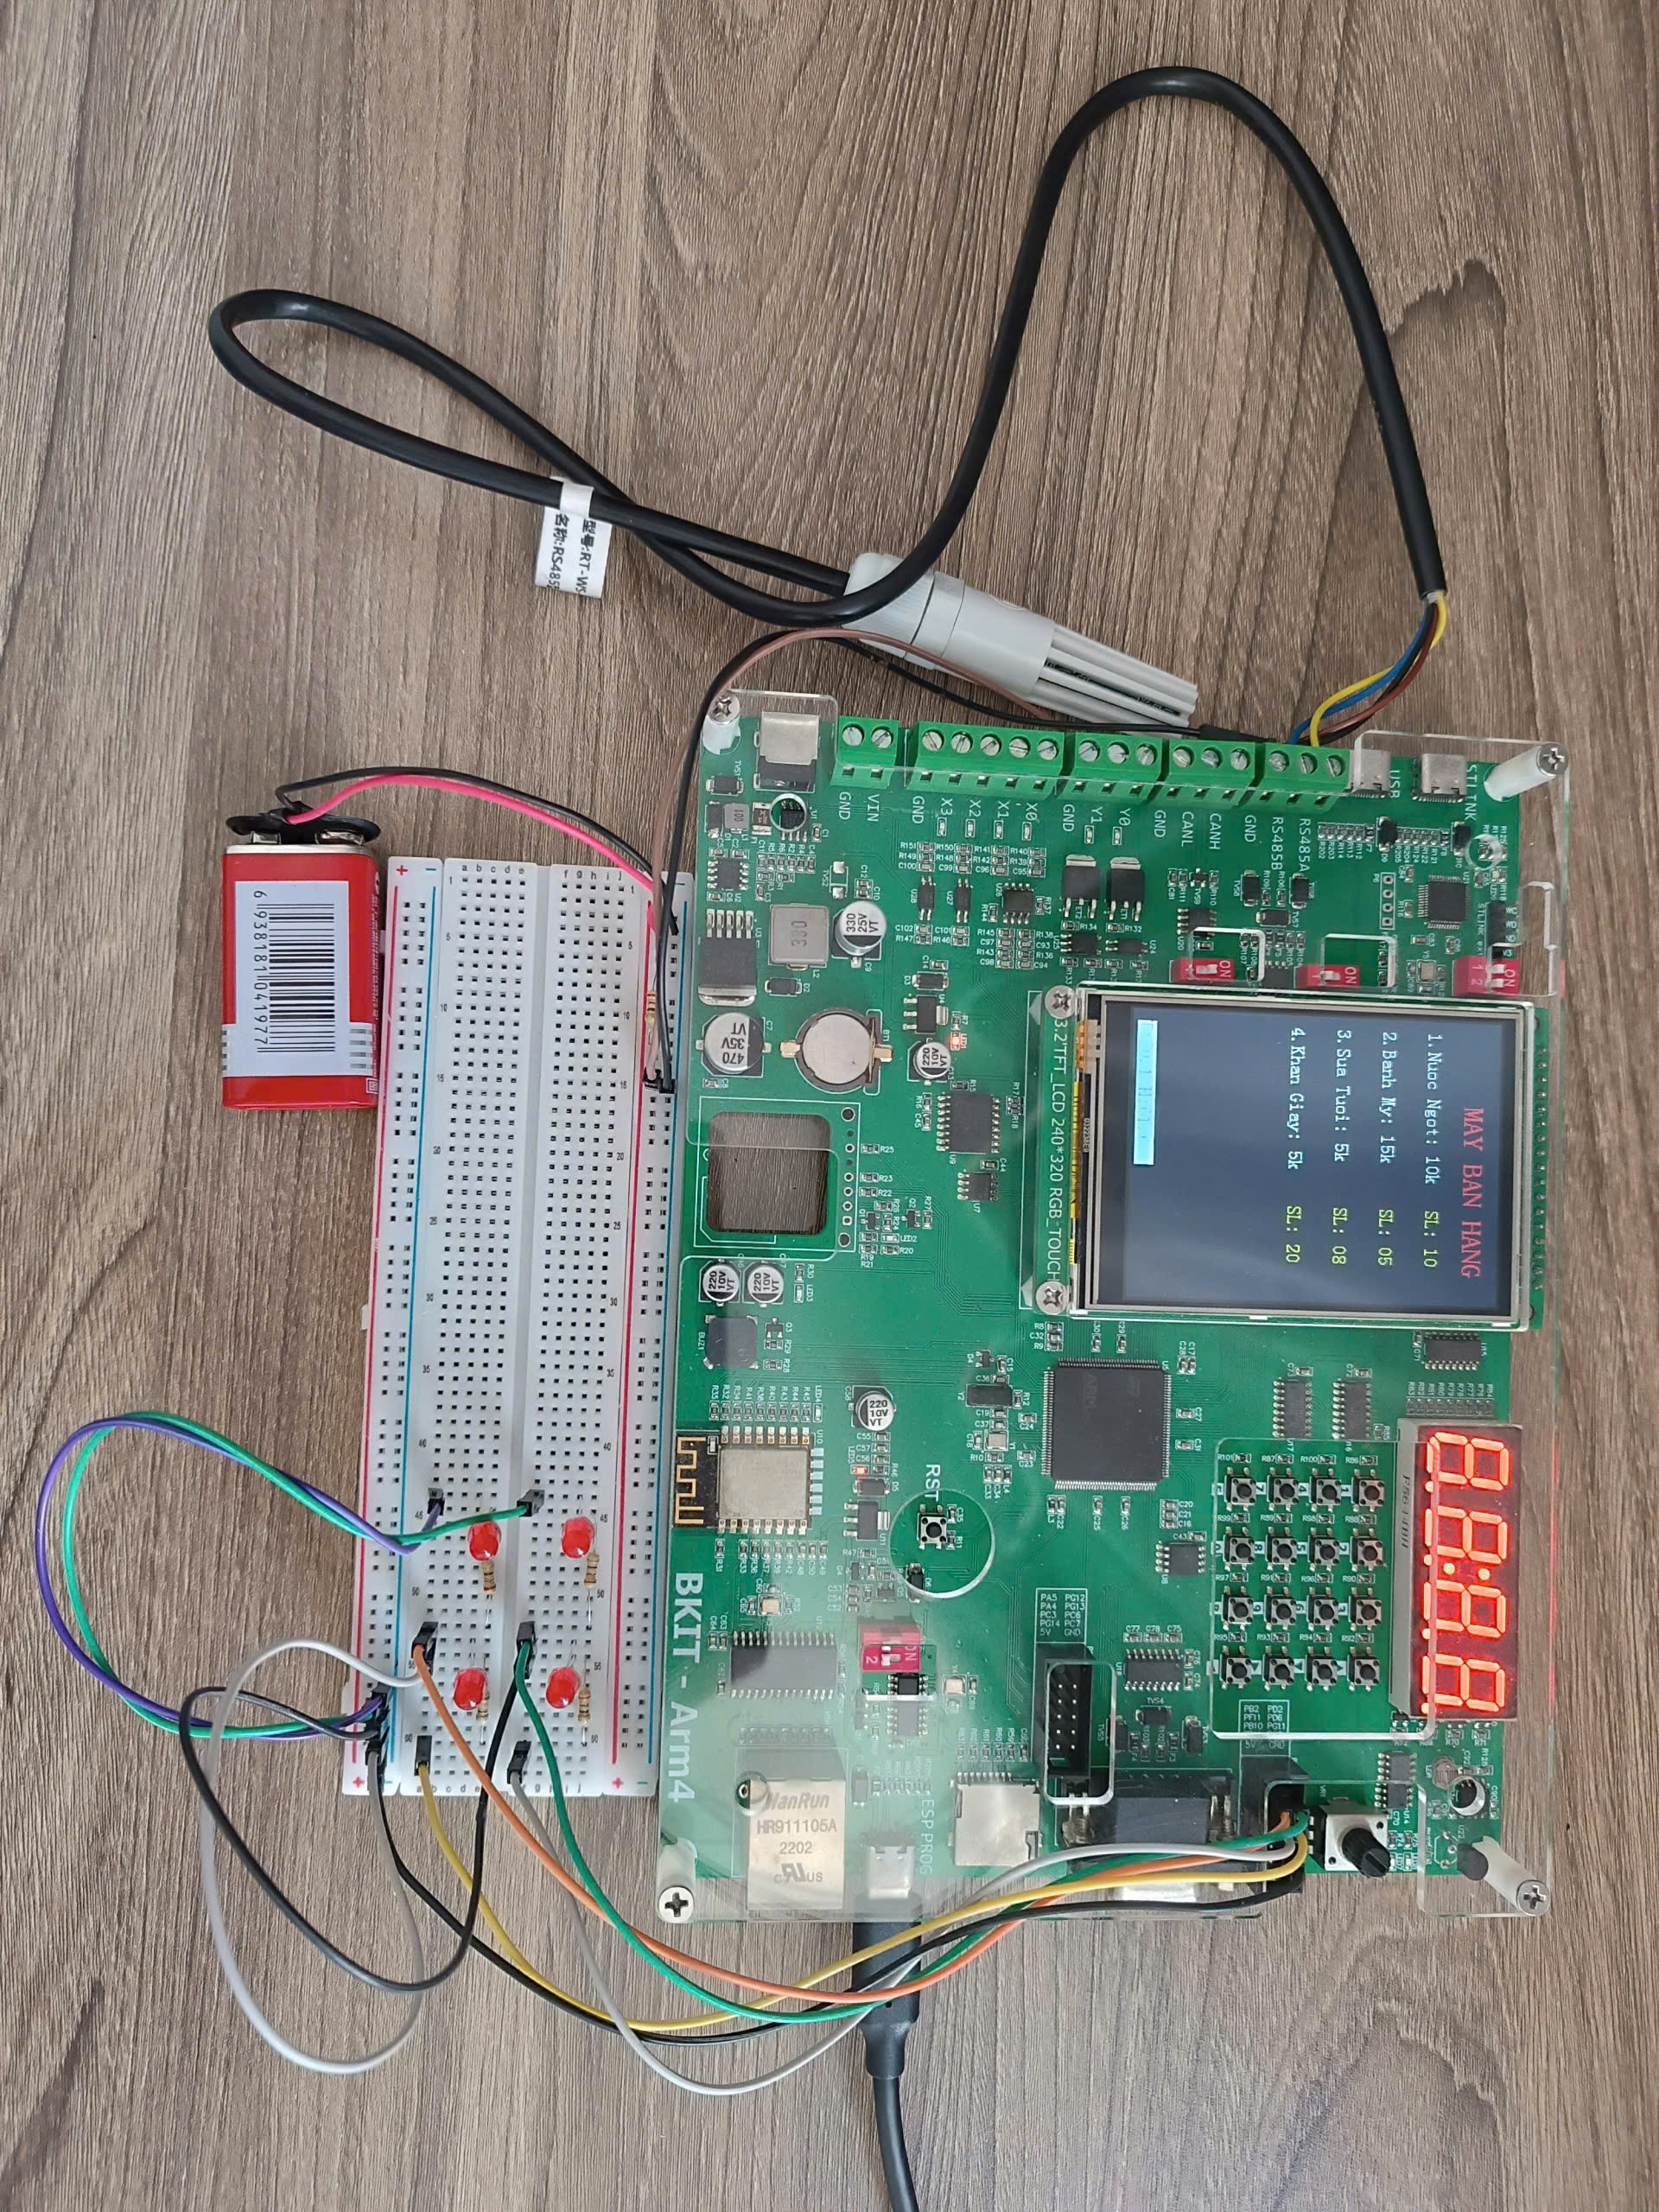
\includegraphics[width=0.7\linewidth, angle=90]{Pics/anhchupthuctehethong.png}
    \caption{Ảnh chụp thực tế hệ thống}
    \label{fig:placeholder}
\end{figure}



\newpage

\subsection{Hiện thực Firmware STM32 (Hệ thống nhúng)}
Firmware được xây dựng dựa trên kiến trúc \textbf{Super Loop kết hợp Software Timer}, đảm bảo khả năng phản hồi thời gian thực mềm (Soft Real-time).
\subsubsection{Kiến trúc Bộ lập lịch (Cooperative Scheduler)}
Hệ thống không sử dụng hàm \texttt{HAL\_Delay()} trong vòng lặp chính để tránh lãng phí chu kỳ máy. Thay vào đó, một thư viện \texttt{software\_timer} được xây dựng dựa trên ngắt Timer phần cứng (TIM2, chu kỳ 10ms).
\begin{itemize}
    \item \textbf{Nguyên lý:} Trong ngắt Timer, các biến đếm lùi được cập nhật. Khi biến đếm về 0, một cờ hiệu (Flag) được bật lên.
    \item \textbf{Hoạt động:} Vòng lặp \texttt{while(1)} liên tục kiểm tra các cờ hiệu này để kích hoạt các tác vụ (Task) tương ứng:
    
    \texttt{button\_scan()}: Chu kỳ 50ms (Đảm bảo chống rung phím).\\
    \texttt{Sensor\_Process\_Task()}: Chu kỳ 5000ms.\\
    \texttt{UART\_Process\_Queue()}: Chu kỳ 100ms (Gửi dữ liệu ra ESP8266).
\end{itemize}
\subsubsection{Máy trạng thái bán hàng (Vending Machine FSM)}
Logic bán hàng được hiện thực hóa bằng mô hình máy trạng thái hữu hạn (FSM) để quản lý luồng hoạt động phức tạp.
\begin{itemize}
    \item \textbf{Quản lý trạng thái:} Sử dụng cấu trúc \texttt{switch-case} để xử lý các trạng thái: \texttt{IDLE, ITEM\_SELECTED, GETTING\_PAYMENT, DISPENSING}.
    \item \textbf{Xử lý sự kiện:} Tại mỗi trạng thái, hệ thống chỉ phản hồi với các sự kiện nút bấm hợp lệ (Ví dụ: Tại trạng thái \texttt{IDLE} chỉ nhận phím chọn món, bỏ qua phím nạp tiền). Điều này ngăn chặn các lỗi logic và hành vi không xác định của người dùng.
\end{itemize}
\subsubsection{Cơ chế chống nghẽn cổ chai UART (UART Circular Buffer)}
Do tốc độ xử lý của ESP8266 (gửi HTTPS) chậm hơn tốc độ gửi dữ liệu của STM32, hiện tượng mất dữ liệu rất dễ xảy ra khi gửi liên tiếp.
\begin{itemize}
    \item \textbf{Giải pháp:} Xây dựng một hàng đợi vòng (Circular Buffer) đóng vai trò bộ đệm trung gian.
    \item \textbf{Hoạt động:} Khi có sự kiện (ví dụ: khởi động lại, cập nhật kho), STM32 đẩy các gói tin vào hàng đợi (Push). Một tác vụ nền (\texttt{UART\_Process\_Queue}) sẽ kiểm tra hàng đợi và lấy từng gói tin ra gửi đi với tốc độ được kiểm soát (Throttling), đảm bảo ESP8266 có đủ thời gian xử lý từng gói tin.
\end{itemize}



\newpage

\subsection{Hiện thực Firmware Gateway (ESP8266)}
ESP8266 đóng vai trò cầu nối (Bridge) thông minh, chịu trách nhiệm phân tích dữ liệu và đồng bộ hóa với Cloud.
\subsubsection{Kỹ thuật xử lý chuỗi dữ liệu (Data Parsing)}
Để khắc phục hiện tượng "Dính gói tin" (Packet Merging) - khi nhiều gói tin UART đến cùng lúc bị gộp thành một chuỗi duy nhất, firmware áp dụng cơ chế đọc theo dòng (Line-by-Line Processing).
\begin{itemize}
    \item \textbf{Cấu hình:} Tăng kích thước bộ đệm nhận \texttt{Serial.setRxBufferSize(1024)} để tránh tràn bộ nhớ khi STM32 gửi dữ liệu dồn dập.
    \item \textbf{Xử lý:} Sử dụng hàm \texttt{Serial.readStringUntil('$\textbackslash$n')} để tách luồng dữ liệu thành từng lệnh riêng biệt dựa trên ký tự kết thúc dòng $\textbackslash$n.
\end{itemize}
\subsubsection{Giao thức định danh gói tin}
Firmware thực hiện phân loại gói tin dựa trên Header (Tiêu đề) để định tuyến dữ liệu lên đúng nhánh cơ sở dữ liệu:
\begin{itemize}
    \item Nếu gói tin bắt đầu bằng \texttt{ENV}: $\to$ Phân tích chuỗi phía sau, tách lấy giá trị Nhiệt độ/Độ ẩm $\to$ Đẩy lên nhánh \texttt{/sensor.}
    \item Nếu gói tin bắt đầu bằng \texttt{STK}: $\to$ Phân tích chuỗi, tách lấy ID và Số lượng $\to$ Đẩy lên nhánh \texttt{/vending\_machine}.
\end{itemize}
\subsection{Hiện thực Web Dashboard (IoT Application)}
Ứng dụng Web được xây dựng theo mô hình \textbf{Serverless} (không máy chủ backend), giao tiếp trực tiếp với Firebase.
\subsubsection{Cơ sở dữ liệu thời gian thực (Realtime Database)}
 Dữ liệu được tổ chức dưới dạng cấu trúc cây JSON (JSON Tree) phẳng hóa để tối ưu tốc độ truy xuất và giảm độ trễ đồng bộ.
\begin{figure}[H]
    \centering
    \includegraphics[width=0.8\linewidth]{Pics/jsontrenfirebaseconsole.png}
    \caption{Cấu trúc JSON trên Firebase Console}
    \label{fig:placeholder}
\end{figure}



\newpage

Giải thích cấu trúc dữ liệu:
\begin{itemize}
    \item \textbf{Nhánh} \texttt{/sensor}: Lưu trữ biến đơn (\texttt{temp}, \texttt{humi}) đại diện cho nhiệt độ và độ ẩm.
    \item \textbf{Nhánh} \texttt{/vending\_machine}: Lưu trữ mảng trạng thái kho hàng (\texttt{item\_0}, \texttt{item\_1},...) đại diện cho số lượng tồn kho của từng món.
\end{itemize}

\subsubsection{Giao diện và Logic (Frontend)}
\begin{itemize}
    \item \textbf{Giao diện (UI):} Sử dụng \textbf{Bootstrap 5} để xây dựng giao diện đáp ứng (Responsive), hiển thị tốt trên cả máy tính và điện thoại. Các thẻ thông tin (Card) được thiết kế đổi màu động (Xanh/Vàng/Đỏ) dựa trên ngưỡng dữ liệu (ví dụ: Tồn kho < 2 chuyển sang màu vàng).
    \item \textbf{Đồng bộ dữ liệu:} Sử dụng \textbf{Firebase SDK} với cơ chế lắng nghe sự kiện \texttt{onValue}. Thay vì phải tải lại trang (Polling), Web App duy trì một kết nối WebSocket với Google Server. Ngay khi ESP8266 cập nhật dữ liệu lên Cloud, sự kiện \texttt{onValue} được kích hoạt, JavaScript sẽ tự động cập nhật DOM (Document Object Model) để thay đổi số liệu trên màn hình ngay lập tức.
\end{itemize}

\subsection{Tổ chức mã nguồn và Giải thích chức năng}
Hệ thống phần mềm được tổ chức theo kiến trúc phân lớp (Layered Architecture) để dễ dàng quản lý và bảo trì. Mã nguồn được chia thành 3 tầng chính: Tầng Ứng dụng (Application), Tầng Điều khiển thiết bị (Driver/Middleware), và Tầng Tiện ích (Utility).\\

Dưới đây là danh sách các file mã nguồn chính và chức năng của chúng:\\

\textbf{1. Tầng Ứng dụng (Application Layer)}\\

Đây là tầng chứa logic nghiệp vụ chính của hệ thống, xử lý luồng hoạt động của máy bán hàng và cảm biến.
\paragraph{\texttt{main.c:}}
\begin{itemize}
    \item \textbf{Chức năng:} Là điểm khởi đầu của chương trình. Chịu trách nhiệm khởi tạo toàn bộ phần cứng (Clock, GPIO, UART, Timer, LCD, Button).
    \item \textbf{Logic:} Chứa vòng lặp vô hạn \texttt{while(1)} đóng vai trò là \textbf{Bộ lập lịch (Scheduler)}, gọi các tác vụ \texttt{Vending\_Loop()} và \texttt{Sensor\_Process\_Task()} hoạt động song song theo cơ chế không chặn (Non-blocking).
\end{itemize}
\paragraph{\texttt{app\_vending.c (.c/.h):}}
\begin{itemize}
    \item \textbf{Chức năng:} Chứa toàn bộ logic điều khiển máy bán hàng tự động.
    \item \textbf{Logic:} Hiện thực máy trạng thái hữu hạn (FSM) với các trạng thái: \texttt{IDLE} (Chờ), \texttt{ITEM\_SELECTED} (Chọn món), \texttt{GETTING\_PAYMENT} (Nạp tiền), \texttt{DISPENSING} (Trả hàng). Quản lý cơ sở dữ liệu sản phẩm (Tên, Giá, Tồn kho) và xử lý giao tiếp gửi cập nhật kho hàng (\texttt{STK}:...) sang ESP8266.
\end{itemize}



\newpage

\paragraph{\texttt{app\_sensor.c (.c/.h):}}
\begin{itemize}
    \item \textbf{Chức năng:} Quản lý tác vụ đọc và gửi dữ liệu môi trường.
    \item \textbf{Logic:} Định kỳ (mỗi 5 giây) gọi hàm đọc cảm biến SHTC3. Sau đó hiển thị nhiệt độ/độ ẩm lên LCD và đóng gói gói tin (\texttt{ENV}:...) gửi sang ESP8266 để đẩy lên Cloud.
\end{itemize}

\textbf{2. Tầng Điều khiển thiết bị (Driver Layer)}\\

Tầng này tương tác trực tiếp với phần cứng của Kit BKIT-ARM4.
\paragraph{\texttt{modbus\_shtc3.c (.c/.h)}:}
\begin{itemize}
    \item \textbf{Chức năng:} Driver giao tiếp với cảm biến SHTC3 qua chuẩn Modbus RTU (RS485).
    \item \textbf{Logic:} Xây dựng khung truyền Modbus (Slave ID, Function Code 0x03), điều khiển chân DE/RE để chuyển đổi hướng truyền/nhận RS485, và gọi hàm tính CRC để kiểm tra toàn vẹn dữ liệu nhận về.
\end{itemize}
\paragraph{\texttt{button.c (.c/.h)}:}
\begin{itemize}
    \item \textbf{Chức năng:} Driver điều khiển ma trận nút nhấn.
    \item \textbf{Logic:} Thay vì đọc GPIO trực tiếp, file này sử dụng giao tiếp \textbf{SPI} để đọc dữ liệu từ IC ghi dịch \textbf{74HC165}. Nó xử lý việc chống rung phím (Debounce) và cập nhật trạng thái nhấn vào mảng \texttt{button\_count[]}.
\end{itemize}
\paragraph{\texttt{lcd.c (.c/.h)}:}
\begin{itemize}
    \item \textbf{Chức năng:} Driver điều khiển màn hình TFT LCD (Chip ILI9341).
    \item \textbf{Logic:} Sử dụng giao tiếp \textbf{FSMC (Flexible Static Memory Controller)} để ghi lệnh và dữ liệu hình ảnh vào bộ nhớ màn hình với tốc độ cao. Cung cấp các hàm vẽ cơ bản: \texttt{lcd\_clear}, \texttt{lcd show\_string}, \texttt{lcd\_draw\_image}.
\end{itemize}
\textbf{3. Tầng Tiện ích (Utility Layer)}\\

Chứa các thư viện bổ trợ dùng chung cho toàn hệ thống.
\paragraph{\texttt{software\_timer.c (.c/.h)}:}
\begin{itemize}
    \item \textbf{Chức năng:} Tạo bộ định thời mềm (Software Timer).
    \item \textbf{Logic:} Dựa trên ngắt phần cứng (Timer Tick) để giảm biến đếm thời gian. Cung cấp cơ chế định thời (ví dụ: 5s đọc cảm biến 1 lần) mà không cần dùng hàm \texttt{HAL\_Delay()} gây treo CPU, giúp hệ thống hoạt động đa nhiệm mượt mà.
\end{itemize}
\paragraph{\texttt{modbus\_crc.c (.c/.h)}:}
\begin{itemize}
    \item \textbf{Chức năng:} Tính toán mã kiểm tra lỗi CRC16.
    \item \textbf{Logic:} Hiện thực thuật toán CRC-16 (Modbus) dựa trên đa thức \texttt{0xA001}, dùng để đảm bảo dữ liệu truyền nhận giữa STM32 và cảm biến không bị sai lệch do nhiễu.
\end{itemize}



\newpage

\renewcommand{\arraystretch}{1.5} % 1.5 nghĩa là cao gấp 1.5 lần bình thường
\begin{longtable}{|
    >{\raggedright\arraybackslash}p{3.5cm}|   % Cột 1: Tên File
    >{\raggedright\arraybackslash}p{2.5cm}|   % Cột 2: Phân loại
    >{\raggedright\arraybackslash}p{5.0cm}|   % Cột 3: Chức năng chính
    >{\raggedright\arraybackslash}p{4.0cm}|   % Cột 4: Giao tiếp phần cứng
|}

\caption{Danh sách các file mã nguồn (Source Code Files):} \label{tab:source_code_files} \\
\hline
\textbf{Tên File} & \textbf{Phân loại} & \textbf{Chức năng chính} & \textbf{Giao tiếp phần cứng} \\
\hline
\endfirsthead

\multicolumn{4}{c}{{\bfseries \tablename\ \thetable{} -- tiếp theo từ trang trước}} \\
\hline
\textbf{Tên File} & \textbf{Phân loại} & \textbf{Chức năng chính} & \textbf{Giao tiếp phần cứng} \\
\hline
\endhead

\hline \multicolumn{4}{|r|}{{Tiếp tục ở trang sau...}} \\ \hline
\endfoot

\hline
\endlastfoot

% --- Dữ liệu bảng ---
main.c & Hệ thống & Khởi tạo \& Lập lịch (Scheduler) & Toàn bộ \\
\hline
app\_vending.c & Ứng dụng & Logic máy bán hàng \& Admin & UART2 (ESP8266) \\
\hline
app\_sensor.c & Ứng dụng & Quản lý tác vụ cảm biến & UART2 \& UART3 \\
\hline
button.c & Driver & Quét phím ma trận & SPI1 (74HC165) \\
\hline
lcd.c & Driver & Hiển thị hình ảnh/chữ & FSMC \\
\hline
modbus\_shtc3.c & Driver & Giao thức Modbus RTU & UART3 (RS485) \\
\hline
software\_timer.c & Tiện ích & Bộ định thời đa nhiệm & TIM2 (Interrupt) \\
\hline
modbus\_crc.c & Tiện ích & Tính toán Checksum CRC16 & Không \\
\hline

\end{longtable}



\newpage

\section{KIỂM THỬ VÀ ĐÁNH GIÁ}
\fancyhead[R]{\small 5. KIỂM THỬ VÀ ĐÁNH GIÁ}

Chương này trình bày kết quả kiểm thử thực tế của hệ thống, bao gồm các kịch bản kiểm thử chức năng, đánh giá hiệu năng và phân tích các vấn đề kỹ thuật đã giải quyết.
\subsection{Kịch bản kiểm thử (Test Cases)}
Hệ thống đã được kiểm thử qua các kịch bản thực tế để xác minh tính đúng đắn của giải thuật và độ ổn định của phần cứng:
\paragraph{1. Mua hàng thành công:}
\begin{itemize}
    \item \textbf{Thao tác:} Người dùng nhấn nút chọn món (ví dụ: Nước ngọt) $\to$ Nhập tiền giả lập từ bàn phím $\to$ Nhấn xác nhận.
    \item \textbf{Kết quả:} Màn hình LCD hiển thị "Giao hàng", Servo tương ứng quay (LED sáng), số lượng tồn kho trên LCD giảm 1. Đồng thời, số lượng trên Web Dashboard giảm 1 ngay lập tức.
\end{itemize}
\paragraph{2. Cập nhật môi trường:}
\begin{itemize}
    \item \textbf{Thao tác:} Thay đổi nhiệt độ môi trường xung quanh cảm biến (ví dụ: hà hơi nóng vào cảm biến SHTC3).
    \item \textbf{Kết quả:} Giá trị nhiệt độ/độ ẩm trên LCD thay đổi. Web Dashboard cập nhật giá trị mới sau mỗi 5 giây, đồ thị biến thiên theo thời gian thực.
\end{itemize}
\paragraph{3. Stress Test (Khởi động lại):}
\begin{itemize}
    \item \textbf{Thao tác:} Nhấn nút Reset cứng trên mạch khi hệ thống đang chạy.
    \item \textbf{Kết quả:} Hệ thống khởi động lại, tự động gửi toàn bộ dữ liệu 4 món hàng lên Web để đồng bộ trạng thái ban đầu. Không xảy ra hiện tượng mất gói tin nhờ cơ chế Queue và Buffer.
\end{itemize}
\subsection{Kết quả Giao diện Web Dashboard (IoT Result)}
Giao diện giám sát từ xa được thiết kế trực quan, hiển thị đầy đủ các thông số quan trọng của hệ thống theo thời gian thực.

\begin{figure}[H]
    \centering
    \includegraphics[width=0.85\linewidth]{Pics/webdashboard.png}
    \caption{Web Dashboard toàn cảnh}
    \label{fig:placeholder}
\end{figure}



\newpage

\textbf{Mô tả các thành phần trên giao diện:}\\
\textbf{Thẻ Giám sát Môi trường (Environmental Monitor):}Hiển thị \textbf{Nhiệt độ (°C)} và \textbf{Độ ẩm (\%RH)} nhận được từ cảm biến SHTC3. Dữ liệu được cập nhật tự động mỗi 5 giây.\\
\textbf{Thẻ Quản lý Kho hàng (Inventory Status):}Liệt kê danh sách 4 mặt hàng với trạng thái màu sắc trực quan:
\begin{itemize}
    \item \textbf{Màu Xanh:} Số lượng > 5 (Tồn kho an toàn).
    \item \textbf{Màu Vàng:} Số lượng 1-5 (Cảnh báo sắp hết).
    \item \textbf{Màu Đỏ + Hiệu ứng rung:} Số lượng = 0 (Hết hàng - Out of Stock).
\end{itemize}

\subsection{Đánh giá hiệu năng hệ thống}

\textbf{Độ mượt (Responsiveness):} Giao diện LCD phản hồi tức thời với thao tác nút nhấn (< 50ms), không bị trễ (lag) do sử dụng cơ chế Timer ngắt quãng thay vì delay cứng.\\
\textbf{Độ tin cậy IoT (Reliability):} Dữ liệu IoT có độ trễ thấp (< 2 giây từ khi bấm nút đến khi Web nhảy số), độ tin cậy cao nhờ giao thức định danh \texttt{STK/ENV} và cơ chế kiểm tra lỗi CRC16. 

\subsection{Các khó khăn gặp phải và giải pháp khắc phục}
Trong quá trình thực hiện đồ án, nhóm đã gặp phải một số vấn đề kỹ thuật phát sinh từ đặc thù phần cứng và giao thức truyền thông. Dưới đây là các khó khăn chính và giải pháp đã áp dụng:

\paragraph{1. Hiện tượng dính gói tin (Packet Merging) trên UART}
\begin{itemize}
    \item \textbf{Vấn đề:} Khi vi điều khiển STM32 gửi liên tiếp nhiều gói tin, module ESP8266 nhận được một chuỗi dữ liệu dài dính liền nhau (VD: \texttt{STK:0,10STK:1,5}...), gây lỗi phân tích.
    \item \textbf{Giải pháp:} Chuyển sang cơ chế xử lý đọc từng dòng (\textbf{Line-by-Line}) trên ESP8266 kết hợp tăng kích thước bộ đệm nhận (RX Buffer) lên 1024 byte.
\end{itemize}
\paragraph{2. Vấn đề nghẽn cổ chai khi khởi động lại hệ thống}
\begin{itemize}
    \item \textbf{Vấn đề:} Khi khởi động, STM32 gửi dồn dập dữ liệu làm tràn bộ đệm ESP8266 (do tốc độ xử lý HTTPS chậm hơn UART).
    \item \textbf{Giải pháp:} Xây dựng cơ chế \textbf{Hàng đợi vòng (Circular Buffer Queue)} trên STM32. Các gói tin được đưa vào hàng đợi và gửi đi từ từ với tốc độ được kiểm soát (Throttling) 100ms/gói.
\end{itemize}
\paragraph{3. Nhiễu tín hiệu trên đường truyền cảm biến RS485}
\begin{itemize}
    \item \textbf{Vấn đề:} Giá trị cảm biến đôi khi bị sai lệch do nhiễu đường dây.
    \item \textbf{Giải pháp:} Hiện thực đầy đủ giải thuật \textbf{CRC-16 (Modbus)} để kiểm tra toàn vẹn dữ liệu. Gói tin lỗi sẽ bị loại bỏ ngay lập tức.
\end{itemize}
\paragraph{4. Xung đột tài nguyên khi quét phím và hiển thị LCD}
\begin{itemize}
    \item \textbf{Vấn đề:} Hàm \texttt{HAL\_Delay()} làm treo CPU, gây khựng màn hình khi bấm phím.
    \item \textbf{Giải pháp:} Loại bỏ hoàn toàn \texttt{HAL\_Delay()} trong vòng lặp chính. Chuyển sang kiến trúc \textbf{Non-blocking} sử dụng thư viện \texttt{software\_timer} để chia nhỏ thời gian xử lý cho từng tác vụ.
\end{itemize}



\newpage

\section{KẾT LUẬN VÀ HƯỚNG PHÁT TRIỂN}
\fancyhead[R]{\small 6. KẾT LUẬN VÀ HƯỚNG PHÁT TRIỂN}

\subsection{Kết luận}
Sau quá trình nghiên cứu và thực hiện, đồ án đã hoàn thành trọn vẹn các mục tiêu đề ra, xây dựng thành công hệ thống \textbf{Máy bán hàng tự động tích hợp IoT} trên nền tảng Kit thí nghiệm BKIT-ARM4.

Những kết quả nổi bật mà nhóm đã đạt được bao gồm:

\paragraph{1. Về mặt hệ thống:}
 Xây dựng thành công mô hình hoạt động ổn định, kết hợp nhịp nhàng giữa vi điều khiển STM32F407 (xử lý trung tâm), module ESP8266 (cầu nối Internet) và các ngoại vi (Cảm biến, LCD, Nút nhấn).
\paragraph{2. Về mặt kỹ thuật phần mềm:}
\begin{itemize}
    \item Áp dụng thành công kiến trúc phần mềm \textbf{Non-blocking} với bộ lập lịch (Scheduler) tự xây dựng, giúp hệ thống phản hồi tức thời ngay cả khi đang thực hiện các tác vụ mạng.
    \item Giải quyết triệt để vấn đề "nghẽn cổ chai" và "dính gói tin" trong giao tiếp UART tốc độ cao bằng cơ chế \textbf{Hàng đợi vòng (Circular Buffer)} và kỹ thuật xử lý chuỗi theo dòng \textbf{(Line-by-Line Parsing)}.
    \item Hiện thực hóa máy trạng thái hữu hạn (FSM) giúp luồng hoạt động của máy bán hàng logic, chặt chẽ và dễ dàng mở rộng.
\end{itemize}
\paragraph{3. Về mặt IoT:}
 Hệ thống giám sát được nhiệt độ/độ ẩm và tồn kho theo thời gian thực (Real-time) trên Web Dashboard với độ trễ thấp (< 2 giây).
 
\subsection{Hạn chế của đề tài}
Bên cạnh những kết quả đạt được, đồ án vẫn còn một số hạn chế do giới hạn về phần cứng và phạm vi nghiên cứu:
\begin{itemize}
    \item \textbf{Cơ chế thanh toán mô phỏng:} Hệ thống hiện tại chỉ mô phỏng việc nạp tiền thông qua các nút nhấn (giả lập mệnh giá 5k, 10k...) thay vì sử dụng các module thanh toán thực tế như đầu đọc tiền mặt hay mã QR.
    \item \textbf{Vấn đề bảo mật:} Cơ sở dữ liệu Firebase đang được cấu hình ở chế độ công khai (Public) để phục vụ mục đích demo, chưa tích hợp cơ chế xác thực người dùng (Authentication), tiềm ẩn rủi ro nếu triển khai thực tế.
    \item \textbf{Phụ thuộc vào kết nối mạng:} Hệ thống chưa có cơ chế lưu trữ cục bộ (Offline Mode). Trong trường hợp mất kết nối WiFi, dữ liệu giao dịch và cảm biến trong thời gian đó sẽ không được đồng bộ và có thể bị mất.
\end{itemize}



\newpage

\subsection{Hướng phát triển}
Để nâng cấp hệ thống trở thành một sản phẩm hoàn thiện hơn và có tính ứng dụng thực tiễn cao, nhóm đề xuất các hướng phát triển sau:
\paragraph{1. Tích hợp thanh toán điện tử:}
 Bổ sung tính năng hiển thị mã QR động (VietQR) trên màn hình LCD. Người dùng có thể quét mã bằng ứng dụng ngân hàng để thanh toán, hệ thống sẽ nhận xác nhận giao dịch qua API ngân hàng (Open Banking).
\paragraph{2. Tăng cường bảo mật:}
\begin{itemize}
    \item Thiết lập lại Firebase Security Rules để chỉ cho phép người dùng đã xác thực mới được quyền ghi dữ liệu.
    \item Xây dựng trang đăng nhập (Login) cho Web Dashboard dành cho người quản trị (Admin).
\end{itemize}
\paragraph{3. Lưu trữ và Báo cáo:}
\begin{itemize}
    \item Sử dụng thẻ nhớ SD (có khe cắm sẵn trên Kit) để lưu nhật ký giao dịch (Log) dưới dạng file \texttt{.txt} hoặc \texttt{.csv}, đảm bảo không mất dữ liệu khi mất mạng.
    \item Nâng cấp Web Dashboard để vẽ biểu đồ doanh thu theo ngày/tháng và biểu đồ biến thiên nhiệt độ môi trường.
\end{itemize}





\section*{TÀI LIỆU THAM KHẢO}


\begin{enumerate}[
    label={[\arabic*]},   
    leftmargin=2em,        
    labelsep=1em,          
    itemsep=0.5\baselineskip
]
    \item Slide bài giảng môn \textbf{Vi xử lý, vi điều khiển - HCMUT}.
    \item Tài liệu hướng dẫn thực hành \textbf{Lab 3: LCD and Button Matrix (BKIT-ARM4)}.
    \item Tài liệu hướng dẫn thực hành \textbf{Lab 8: ESP8266 - WIFI (BKIT-ARM4)}.
    \item Datasheet: \textbf{STM32F407, SHTC3 Sensor, ILI9341 Driver}.
    \item ABC Solutions. (n.d.). \textit{Kit Thí nghiệm BKIT ARM 4}. Truy cập từ: \href{https://abcsolutions.com.vn/index.php/kit-thi-nghiem-bkit-arm4/}{\textbf{ABC Solutions: Kit thí nghiệm BKIT-ARM4}}
\end{enumerate}

\end{document}  
